%%%
%
% FIXME: An additional waning crescent moon phase is missing in Question 17!
% The phases shown in Q 14 need to be fixed!
%
% Question 12 is poorly worded. A month from question 10 or a month from
% Question 11?
%
% Kill the age and % illuminated in the last question
%
% Shorten the rise and set table and add some conceptual questions.
%


\documentclass[11pt]{article}
\usepackage{tocloft}
\usepackage{graphicx}
\usepackage{calc}
\usepackage{amssymb}
\usepackage{color}
\usepackage{array}
\usepackage[sc]{mathpazo}
\usepackage{url}
\usepackage[final]{pdfpages}
\usepackage{multirow}

%\linespread{1.05}
\oddsidemargin=0pt
\evensidemargin=0pt
\textwidth=6.5in
\topmargin=0pt
\headheight=0pt
\headsep=0pt
\textheight=9in
% EXPERIMENTAL
%\parindent=0pt
%\parskip=3pt
\setlength{\parindent}{0cm}
\newcommand\secfont{\fontfamily{cmss}\selectfont}%\textwidth 5.5truein
\newcommand\pifheading[1]{{\secfont\textbf{#1}:}}
%\oddsidemargin -0.40truein
%\textheight 8.0truein
%\topmargin -0.25truein
\def\lo{
\mathrel{\raise.3ex\hbox{$<$}\mkern-14mu\lower0.6ex\hbox{$\sim$}}
}
\def\hi{
\mathrel{\raise.3ex\hbox{$>$}\mkern-14mu\lower0.6ex\hbox{$\sim$}}
}

\textwidth = 6.6 in
\textheight = 9.1 in
\oddsidemargin = -0.05 in
\evensidemargin = +0.05 in
\topmargin = -.1 in
\headheight = 0.0 in
\headsep = 0.0 in
\parskip = 0.06in
\newcommand\registered{{\ooalign{\hfil\raise .00ex\hbox{\scriptsize R}\hfil\crcr\mathhexbox20D}}}

%% Define a new 'leo' style for the package that will use a smaller font.
\makeatletter
\def\url@leostyle{%
  \@ifundefined{selectfont}{\def\UrlFont{\sf}}{\def\UrlFont{\small\ttfamily}}}
\makeatother
%% Now actually use the newly defined style.
\urlstyle{leostyle}

%\pagestyle{empty}
%\includeonly{previous,proposal_references}
%\includeonly{proposal_references}
%\includeonly{previous}

% TOC

\begin{document}
%%%%%%%%%%%%%%%%%%%%%%%%%%%%%%%%%%%%%%%%%%%%%%%%%%%%%%%%%%%%%%%%%%%%%
\begin{center}
\textbf{\Large
AST101: Our Corner of the Universe \\
\vspace*{0.1cm}
Lab 2: The Sun and Phases of The Moon
}
\end{center}

\vspace*{0.5cm}

{\Large Name:}\vspace*{0.5cm}\\\hrule
{\Large NetID (your SU email address, without the @syr.edu):}\vspace*{0.5cm}\\\hrule
{\Large Lab section number:}\vspace*{0.5cm}\\\hrule
\vspace*{0.5cm}

%%%%%%%%%%%%%%%%%%%%%%%%%%%%%%%%%%%%%%%%%%%%%%%%%%%%%%%%%%%%%%%%%%%%%
\section{Introduction}

\subsection*{Objectives} 

The first part of this lab uses the Paths of the Sun Simulator to explore the
seasonal changes in the Sun's path through the sky. The second part of the lab
uses lunar simulators to explore the phases of the Moon seen from the Earth.

\subsection*{Materials}

Links to the animations required for this lab are available at \\
\\
\url{https://walterfreeman.github.io/ast101/labs.html}

\section{Seasonal Changes in the Sun's Motion}

\subsection{Introduction to the Motions of the Sun Simulator}

This simulator allows you to simulate the path of the sun for any date during the year for any latitude on the Earth. Spend some time familiarizing yourself with the simulator. Most of the controls are fairly intuitive and similar to those in the preceding lab. 

\begin{itemize}
\item	Practice using the yearly slider to move to different dates during the year.
\item	Practice using the map to move to different latitudes during the year. 
\item	Note that the simulation lists the right ascension, declination, azimuth, and altitude for the sun at all times. 
\item	Note that some advanced features such as the sidereal time, hour angle, equation of time, and the analemma are available in a box in the lower left in this simulation, but will not be used in this lab. 
\item	Note that there are three different animation modes. 
\begin{itemize}
\item	If you select continuous, time will move forward in a natural fashion. You may adjust the rate at which time passes using the animation speed slider. You may modify this mode with the loop day check box which will cause the sun's motion for the current day to continually repeat.
\item	 If you select step by day, time will leap forward in 24 hour increments and the time of day will not change. 
\end{itemize}
\item	Special care should be taken to make sure that you understand what is being simulated at all times. This is especially true in regard to discriminating between the yearly and daily motion of the sun. 
\begin{itemize}
\item	Move to a middle United States Latitude like $35^\circ$N. Click show ecliptic and show month labels. This is the sun's yearly path on the celestial sphere and is denoted by a white circle in the simulator. Note that it crosses the blue celestial equator on the equinoxes. 
\item	Change your time to noon (12 pm) and animate the simulator in the step by day mode. The sun's meridional altitude is the sun's altitude angle when it passes through the line on the celestial sphere that joins the North Point to the South point. This line is called the meridian. It is the ``highest'' point that an object will be in the sky. You can watch the changing meridional altitude of the sun throughout the year. 
\item	Stop the simulation near the summer solstice. The simulator readout should state ``The horizon diagram is shown for an observer at latitude $35^\circ$ on 21 June at 12:00 (12:00 pm)''. Think about what the sun's path should look like in the sky on that day. 
\end{itemize}
\end{itemize}

\vspace*{0.5cm}
\noindent
\textbf{Question 1.} Set up the simulator for Syracuse, NY which has a latitude of $43^\circ$~N. The sun's meridional altitude is the sun's altitude angle when it passes through the line on the celestial sphere that joins the North Point to the South point. This line is called the meridian. It is the ``highest'' point that an object will be in the sky. Find the meridian on the simulator. What time is it when the Sun passes through the meridian?
\vspace*{0.8cm}

\hrulefill\\

\vspace*{-0.2cm}
\noindent
\textbf{Question 2.}
Complete the following chart for the meridional altitude and the rising and setting azimuths for the 3 major paths of the sun. Note that the rising azimuth can be determined by dragging the sun (dragging in time of day mode) and reading off the azimuth when the altitude is zero. 

\begin{center}
\begin{tabular}{|l||l|l|l|}
\hline
\textbf{Date} & \textbf{Meridional Altitude} & \textbf{Rising Azimuth} & \textbf{Setting Azimuth} \\\hline\hline
Summer Solstice  & \parbox{0.12\linewidth}{\vspace*{1cm}} & \parbox{0.12\linewidth}{\vspace*{1cm}} & \parbox{0.12\linewidth}{\vspace*{1cm}} \\\hline
Autumnal Equinox & \parbox{0.12\linewidth}{\vspace*{1cm}} & \parbox{0.12\linewidth}{\vspace*{1cm}} & \parbox{0.12\linewidth}{\vspace*{1cm}} \\\hline
Winter Solstice  & \parbox{0.12\linewidth}{\vspace*{1cm}} & \parbox{0.12\linewidth}{\vspace*{1cm}} & \parbox{0.12\linewidth}{\vspace*{1cm}} \\\hline
\end{tabular}
\end{center}
\newpage

\noindent
Now use the results from the table above to help you draw the 3 paths in the horizon diagram below. Label each path. Use your diagram to answer the next four questions.
\vspace*{-0.3cm}
\begin{center}
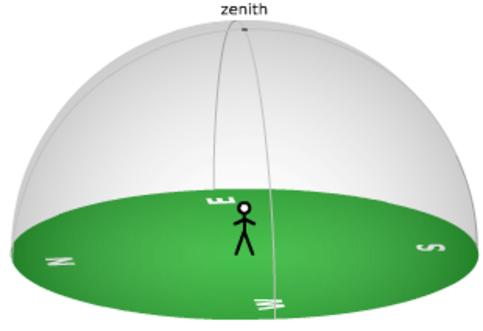
\includegraphics{local_sky}
\end{center}

\noindent
In the summer, does the sun rise north of east, south of east of directly east?
\vspace*{0.5cm}

\hrulefill\\
\noindent

\noindent
In the winter, does the sun rise north of east, south of east of directly east?
\vspace*{0.5cm}

\hrulefill\\
\noindent

\noindent
On what day of the year is the sun \emph{highest} in the sky at noon?
\vspace*{0.5cm}

\noindent
On what day of the year would you get the \emph{least} direct sunlight?
\vspace*{0.5cm}

\hrulefill\\

\noindent
\textbf{Question 3.}
Suppose that you are visiting Syracuse, NY and on July 10 you wake up early and note the rising azimuth of the sun. In which direction would the value change if you measured it two weeks later?
\vspace*{0.5cm}

\hrulefill\\
\noindent
\textbf{Question 4.}
We know that the sun can never be at the zenith for Syracuse (latitude = $43^\circ$~N). How far would you need to move on the Earth to find a latitude where the sun can be at the zenith?
\vspace*{0.5cm}

\enlargethispage*{1000pt}
\hrulefill\\
\newpage
\noindent
\textbf{Question 5.}
Set up the simulator for Nordkaap, Norway which has a latitude of $71^\circ$~N. Complete the following chart for the meridional altitude and the rising and setting azimuths for the 3 major paths of the sun and use these to draw the 3 paths in the horizon diagram below.
\begin{center}
\begin{tabular}{|l||l|l|l|}
\hline
\textbf{Date} & \textbf{Meridional Altitude} & \textbf{Rising Azimuth} & \textbf{Setting Azimuth} \\\hline\hline
Summer Solstice  & \parbox{0.12\linewidth}{\vspace*{1cm}} & \parbox{0.12\linewidth}{\vspace*{1cm}} & \parbox{0.12\linewidth}{\vspace*{1cm}} \\\hline
Autumnal Equinox & \parbox{0.12\linewidth}{\vspace*{1cm}} & \parbox{0.12\linewidth}{\vspace*{1cm}} & \parbox{0.12\linewidth}{\vspace*{1cm}} \\\hline
Winter Solstice  & \parbox{0.12\linewidth}{\vspace*{1cm}} & \parbox{0.12\linewidth}{\vspace*{1cm}} & \parbox{0.12\linewidth}{\vspace*{1cm}} \\\hline
\end{tabular}
\end{center}
\begin{center}
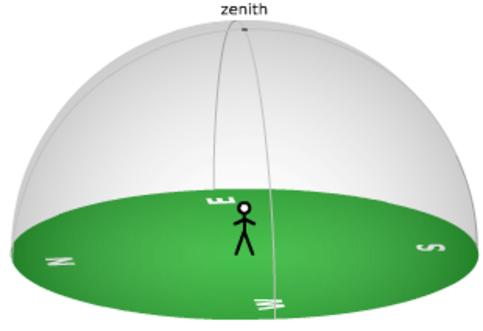
\includegraphics{local_sky}
\end{center}
\newpage

\noindent
\textbf{Question 6.}
Note that the sun doesn't rise every day from Nordkaap. How far would you need to move on the Earth to find a latitude where the sun does rise every day?
\vspace*{1cm}

\hrulefill\\

\vspace*{-0.2cm}
\noindent
\textbf{Question 7.}
The Paths of the Sun Simulator is also very useful for determining how long the sun is above the horizon each day. Simply make sure that the option for dragging the sun's disk is set to time of day and drag the sun to the eastern/western horizon read the clock to determine the time at which the sun rises/sets. 

\begin{center}
\begin{tabular}{|l|l||l|l|l|}
\hline
\textbf{Latitude} & \textbf{Date} & \textbf{Rising Time} & \textbf{Setting Time} & \textbf{Total Time} \\\hline\hline
\multirow{3}{*}{$0^\circ$~N} & June 21 & \parbox{0.12\linewidth}{\vspace*{1cm}} & \parbox{0.12\linewidth}{\vspace*{1cm}} & \parbox{0.12\linewidth}{\vspace*{1cm}} \\\cline{2-5}
& September 21 & \parbox{0.12\linewidth}{\vspace*{1cm}} & \parbox{0.12\linewidth}{\vspace*{1cm}} & \parbox{0.12\linewidth}{\vspace*{1cm}} \\\cline{2-5}
& December 21 & \parbox{0.12\linewidth}{\vspace*{1cm}} & \parbox{0.12\linewidth}{\vspace*{1cm}} & \parbox{0.12\linewidth}{\vspace*{1cm}} \\\cline{1-5}
\multirow{3}{*}{$43^\circ$~N} & June 21 & \parbox{0.12\linewidth}{\vspace*{1cm}} & \parbox{0.12\linewidth}{\vspace*{1cm}} & \parbox{0.12\linewidth}{\vspace*{1cm}} \\\cline{2-5}
& September 21 & \parbox{0.12\linewidth}{\vspace*{1cm}} & \parbox{0.12\linewidth}{\vspace*{1cm}} & \parbox{0.12\linewidth}{\vspace*{1cm}} \\\cline{2-5}
& December 21 & \parbox{0.12\linewidth}{\vspace*{1cm}} & \parbox{0.12\linewidth}{\vspace*{1cm}} & \parbox{0.12\linewidth}{\vspace*{1cm}} \\\cline{1-5}
\multirow{3}{*}{$66.5^\circ$~N} & June 21 & \parbox{0.12\linewidth}{\vspace*{1cm}} & \parbox{0.12\linewidth}{\vspace*{1cm}} & \parbox{0.12\linewidth}{\vspace*{1cm}} \\\cline{2-5}
& September 21 & \parbox{0.12\linewidth}{\vspace*{1cm}} & \parbox{0.12\linewidth}{\vspace*{1cm}} & \parbox{0.12\linewidth}{\vspace*{1cm}} \\\cline{2-5}
& December 21 & \parbox{0.12\linewidth}{\vspace*{1cm}} & \parbox{0.12\linewidth}{\vspace*{1cm}} & \parbox{0.12\linewidth}{\vspace*{1cm}} \\\cline{1-5}
\multirow{3}{*}{$90^\circ$~N} & June 21 & \parbox{0.12\linewidth}{\vspace*{1cm}} & \parbox{0.12\linewidth}{\vspace*{1cm}} & \parbox{0.12\linewidth}{\vspace*{1cm}} \\\cline{2-5}
& September 21 & \parbox{0.12\linewidth}{\vspace*{1cm}} & \parbox{0.12\linewidth}{\vspace*{1cm}} & \parbox{0.12\linewidth}{\vspace*{1cm}} \\\cline{2-5}
& December 21 & \parbox{0.12\linewidth}{\vspace*{1cm}} & \parbox{0.12\linewidth}{\vspace*{1cm}} & \parbox{0.12\linewidth}{\vspace*{1cm}} \\\cline{1-5}

\end{tabular}
\end{center}

\noindent
Based on your answers to the previous questions, is it best to refer to sunlight as a seasonal or daily phenomena? Does this depend on latitude? Explain your answer.

\vspace*{2cm}

\hrulefill\\

\newpage

\section{Phases of The Moon}

\subsection{Introduction to Moon Phases}

Use the background information on moon phases (at \url{http://astro.unl.edu/naap/lps/lunarPage1.html}) 
to answer the questions below.

\noindent
\textbf{Question 8.}
Is there a dark side of the moon?  (Note: this question can be effectively answered either yes or no, so it is important to explain your reasoning.) 
\vspace*{2cm}

\hrulefill\\

\noindent
\textbf{Question 9.}
How much of the Moon's surface is illuminated by the Sun at any time?
\vspace*{1cm}

\hrulefill\\

\noindent
\textbf{Question 10.}
How long does it take the moon to complete one cycle of phases, in days?
\vspace*{1cm}

\hrulefill\\

\noindent
\textbf{Question 11.}
If the moon is full today, what phase do you expect it to be at in a week? 
\vspace*{1cm}

\hrulefill\\

\noindent
\textbf{Question 12.}
How about one month later? Make sure you define what you mean by ``month''!
\vspace*{1cm}

\hrulefill\\

\noindent
\textbf{Question 13.}
Many words in astronomy also non-astronomical uses as well. Using your knowledge of how the terms on the left are used in astronomy match them with the non-astronomical uses on the right.
\vspace*{0.5cm}

\noindent
\hspace*{1cm} waning \hspace*{3cm} convex, rounded---also hunch-backed, having a hump
\vspace*{0.5cm}

\noindent
\hspace*{1cm} gibbous \hspace*{3cm} increasing in size, quantity, volume, intensity, etc.
\vspace*{0.5cm}

\noindent
\hspace*{1cm} waxing \hspace*{3cm} decreasing in magnitude, importance, brilliancy, intensity, etc.

\newpage
\noindent
\textbf{Question 14.}
Order the moon phases
given below correctly, starting with the new moon, passing through the full
moon and back to the new moon again.\\
\vspace*{0.5cm}\\
\hspace*{1cm}\textbf{A\hspace*{6cm} F \hspace*{6cm} A}\\

\hrulefill\\

\begin{center}
\begin{tabular}{|c|c|c|c|c|}\hline
\parbox{1in}{\vspace*{0.1cm}
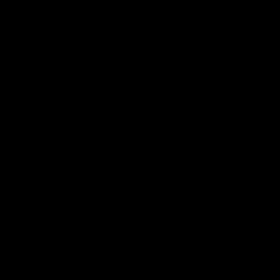
\includegraphics[width=1in]{new}
} & 
\parbox{1in}{\vspace*{0.1cm}
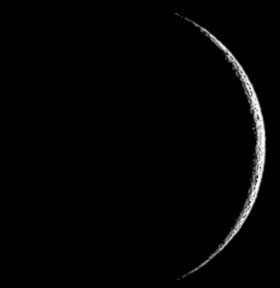
\includegraphics[width=1in]{moon_01}
} & 
\parbox{1in}{\vspace*{0.1cm}
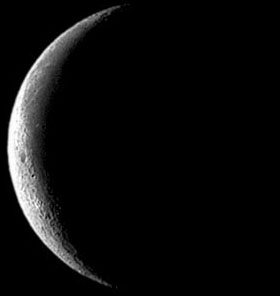
\includegraphics[width=1in]{moon_05}
} & 
\parbox{1in}{\vspace*{0.1cm}
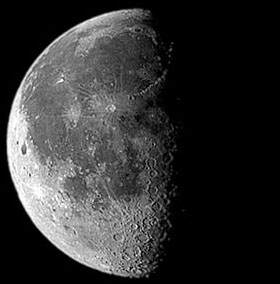
\includegraphics[width=1in]{third_q}
} & 
\parbox{1in}{\vspace*{0.1cm}
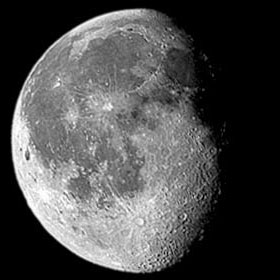
\includegraphics[width=1in]{moon_06}
} \\
\hline
A & B & C & D & E \\\hline\hline
\parbox{1in}{\vspace*{0.1cm}
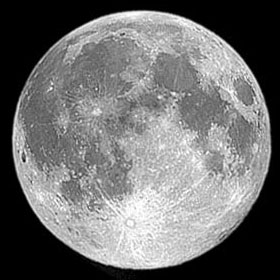
\includegraphics[width=1in]{full}
} & 
\parbox{1in}{\vspace*{0.1cm}
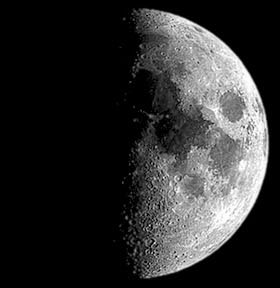
\includegraphics[width=1in]{first_q}
} & 
\parbox{1in}{\vspace*{0.1cm}
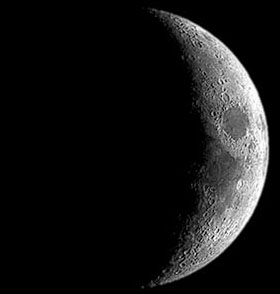
\includegraphics[width=1in]{moon_02}
} & 
\parbox{1in}{\vspace*{0.1cm}
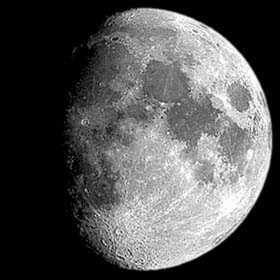
\includegraphics[width=1in]{moon_04}
} & 
\parbox{1in}{\vspace*{0.1cm}
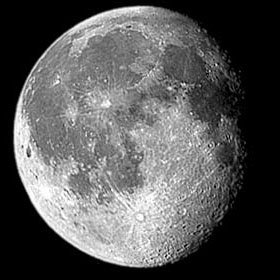
\includegraphics[width=1in]{moon_03}
} \\
\hline
F & G & H & I & J \\\hline
\end{tabular}
\end{center}

\noindent
\textbf{Question 15.} Give the names of the six phases identified by their
letters below. 

\noindent
Phase B:
\vspace*{0.5cm}

\hrulefill\\
\noindent
Phase E:
\vspace*{0.5cm}

\hrulefill\\
\noindent
Phase F:
\vspace*{0.5cm}

\hrulefill\\
\noindent
Phase G:
\vspace*{0.5cm}

\hrulefill\\
\noindent
Phase C:
\vspace*{0.5cm}

\hrulefill\\
\noindent
Phase H:
\vspace*{0.5cm}

\hrulefill\\

\newpage

\subsection{Lunar Phase Simulator}

Use the \emph{Lunar Phase Simulator} to answer the questions below.

\noindent
\textbf{Question 16.} 
From the perspective of an observer above the North Pole, what direction does
the moon move in its orbit around the Earth? (Clockwise or counterclockwise)
\vspace*{0.5cm}

\hrulefill\\
\noindent
\textbf{Question 17.} In the diagram below the sun's light is coming in from the right. The moon's location is marked at several points on its orbit. These are the points the moon was at when the sketches above were drawn. Identify each position with the letter of the corresponding sketch (from the previous page).

\begin{center}
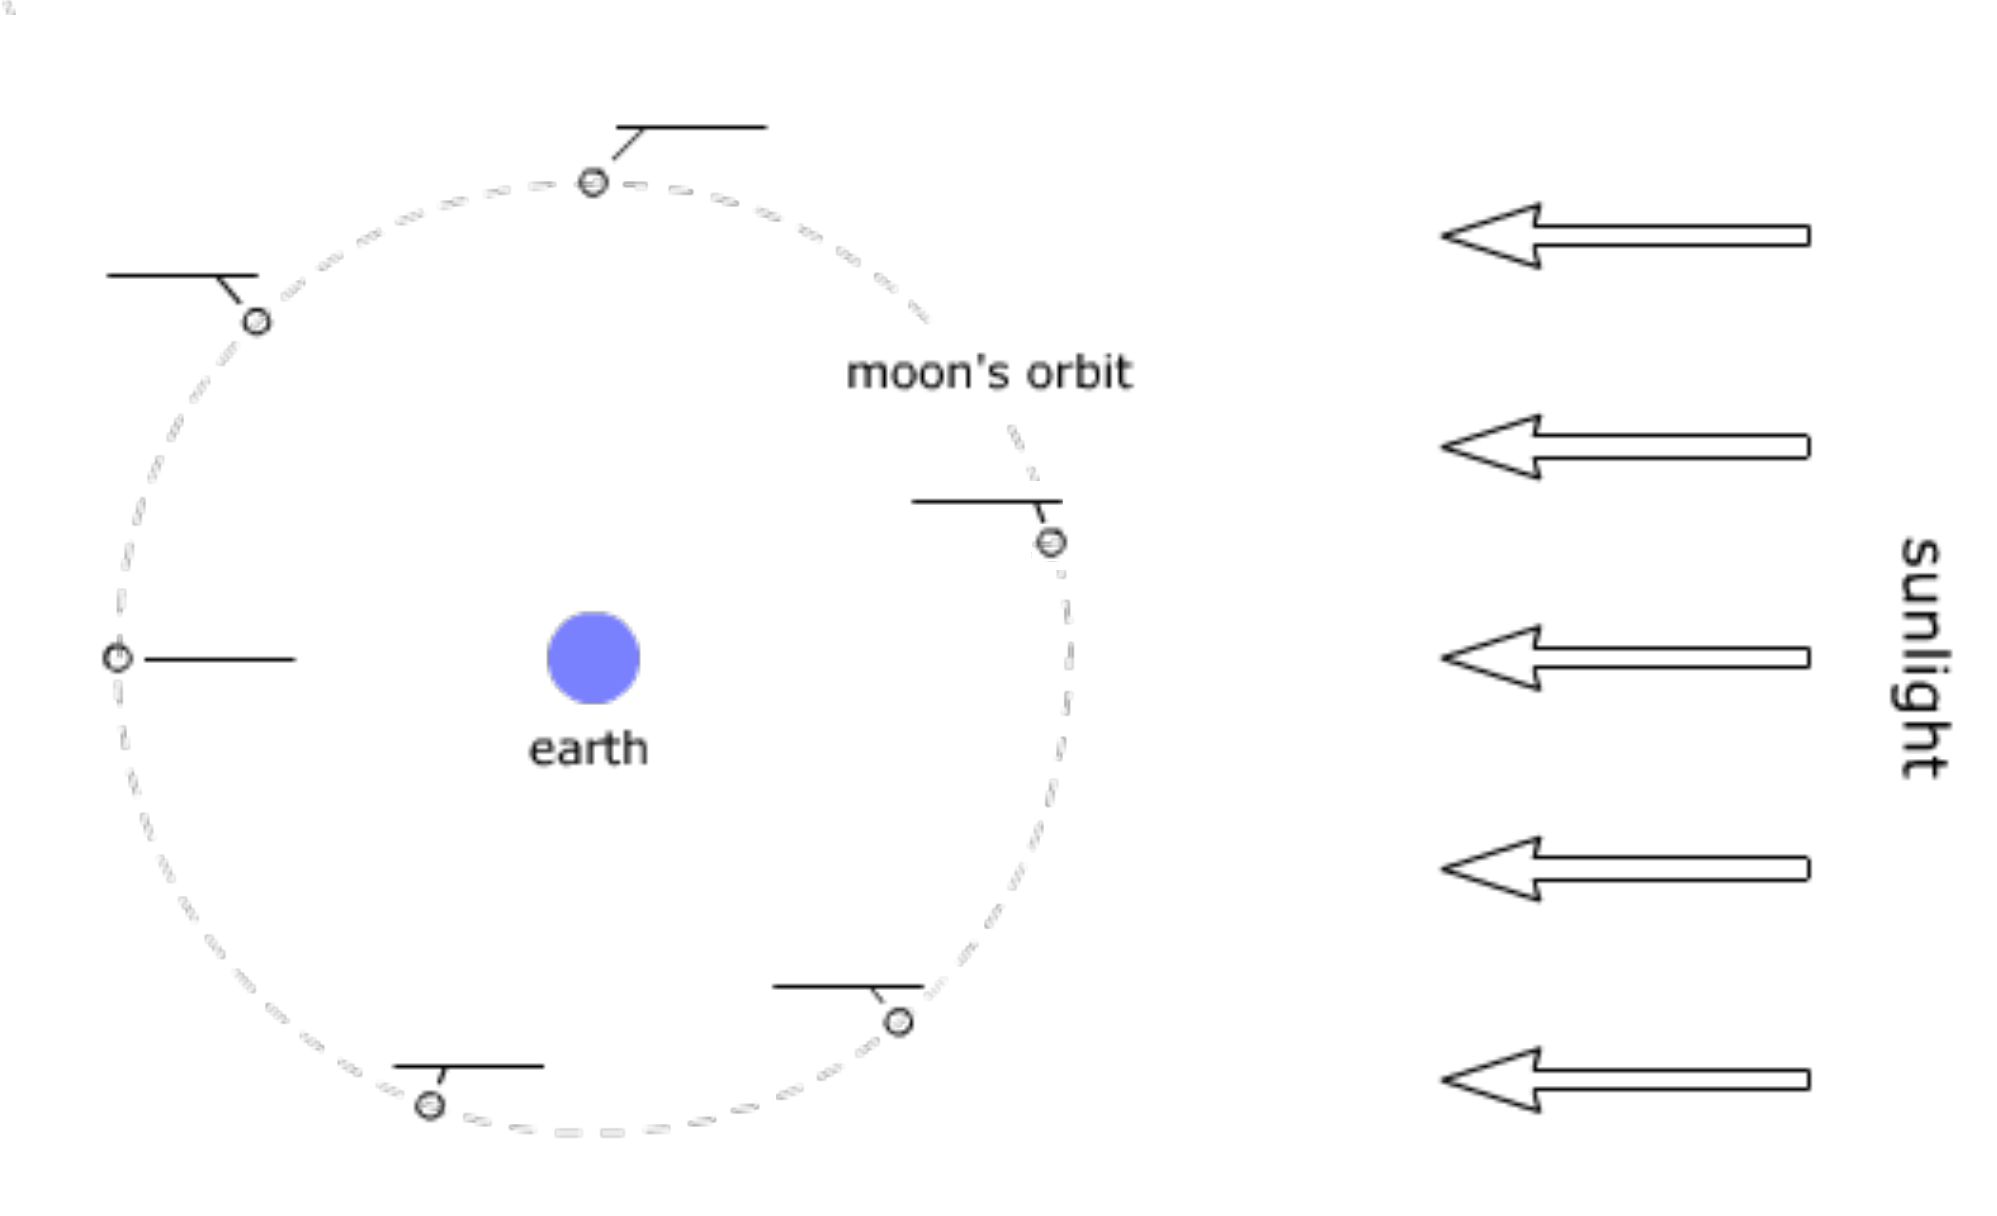
\includegraphics{moon_orbit.png}
\end{center}

\subsection{Visualizing Phases}

Use the \emph{Moon Bisector Demo} to answer the questions below.

\noindent
\textbf{Question 18.} 
We can determine the appearance of the moon based on the orientation of the moon and sun with a simple heuristic.   In the figure below, bisect the moon \emph{twice.} 
\begin{itemize}
\item Draw a line (perpendicular to the direction of sunlight) that shows the half of the entire moon that is illuminated and shade the shadowed region.
\item Draw a line (perpendicular to the Earth-moon line) that shows the half of the moon visible for an observer on earth. 
\item Mark the region that is both visible from earth and illuminated by the sun. That region will be the phase of the moon we on earth see.
\end{itemize}

\newpage

\vspace*{1cm}
\begin{center}
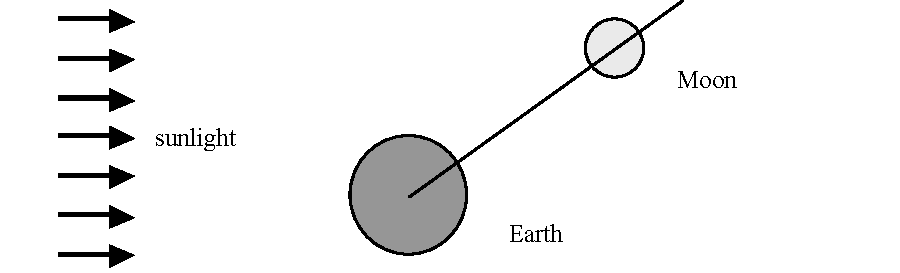
\includegraphics{moon_bisect}
\end{center}
\vspace*{1cm}

\noindent
We normally draw the phases of the moon with the terminator (the dividing line between light and shadow) from the north pole to the south pole of the moon.  This is how the moon would be seen if it were on the observer's meridian.  We can use the drawing above to determine the amount of illumination and whether it is on the left or right hand side of the moon.  Use the drawing above to draw the appearance of the moon in the box below by shading in the portion that is dark.

\begin{center}
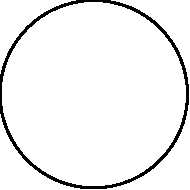
\includegraphics{blank_moon}
\end{center}

\noindent
Open the Moon Bisector Demo and use the simulator to check your answer to the above problem.

\subsection{Working with the Lunar Phase Simulator}

The items below will help familiarize yourself with the controls and usability features of the simulator.
\begin{itemize}
\item	If you have not already done so, launch the Lunar Phase Simulator
\item	The main panel has sunlight, the earth, and moon. The earth and moon can be dragged with the mouse.
\item	Below the main panel, there are animation controls. The moon and earth can be dragged.
\item	The increment buttons move both the moon and earth by the specified time.
\item	The Moon Phase panel shows the current moon phase. Drop down menus will jump to a predefined position. Note that the phases, such as crescent and gibbous, are more broad than the particular point chosen by the presets.
\item	The Horizon Diagram panel displays the point of view of the observer (and you are a second observer looking down on that observer).
\item	The observer's horizon diagram can be dragged to allow for the most convenient viewing orientation.
\item	The sun and moon on the globe can be dragged around.
\item	In the Diagram Options panel, the show angle option shows the earth-moon-sun angle. The phases are technically defined in terms of this angle. 
\item	In the Diagram Options panel, the show lunar landmark option draws a point of reference to more easily observer lunar rotation and revolution.
\item	In the Diagram Options panel, the show time tick-marks option displays the time of day of the observer.
\end{itemize}

\subsection{Understanding the Earth--Moon--Sun System}
\noindent
\textbf{Question 19.} 
Question 9: Click on the option labeled show angle which graphically displays the angle between the direction of the sun and moon.  Now drag the moon around the sun to a variety of different locations and note the appearance of the Moon Phase.  Describe how the value of the angle correlates with the appearance of the moon.


\vspace*{4cm}
\hrulefill\\

\textbf{Question 20.}
Each row in the table on the following page shows diagram of the earth-moon system. For each diagram, find the age of the moon at that position (that is, the time passed since new moon), its phase, and its percent illumination. Finally, make a sketch of its general appearance. You will need to take into account the orientation of the sunlight---it is different in each diagram from the orientation in the applet. The first row is completed for you. You may need to rotate your paper and hold it up to the screen to check your answers.  
\newpage

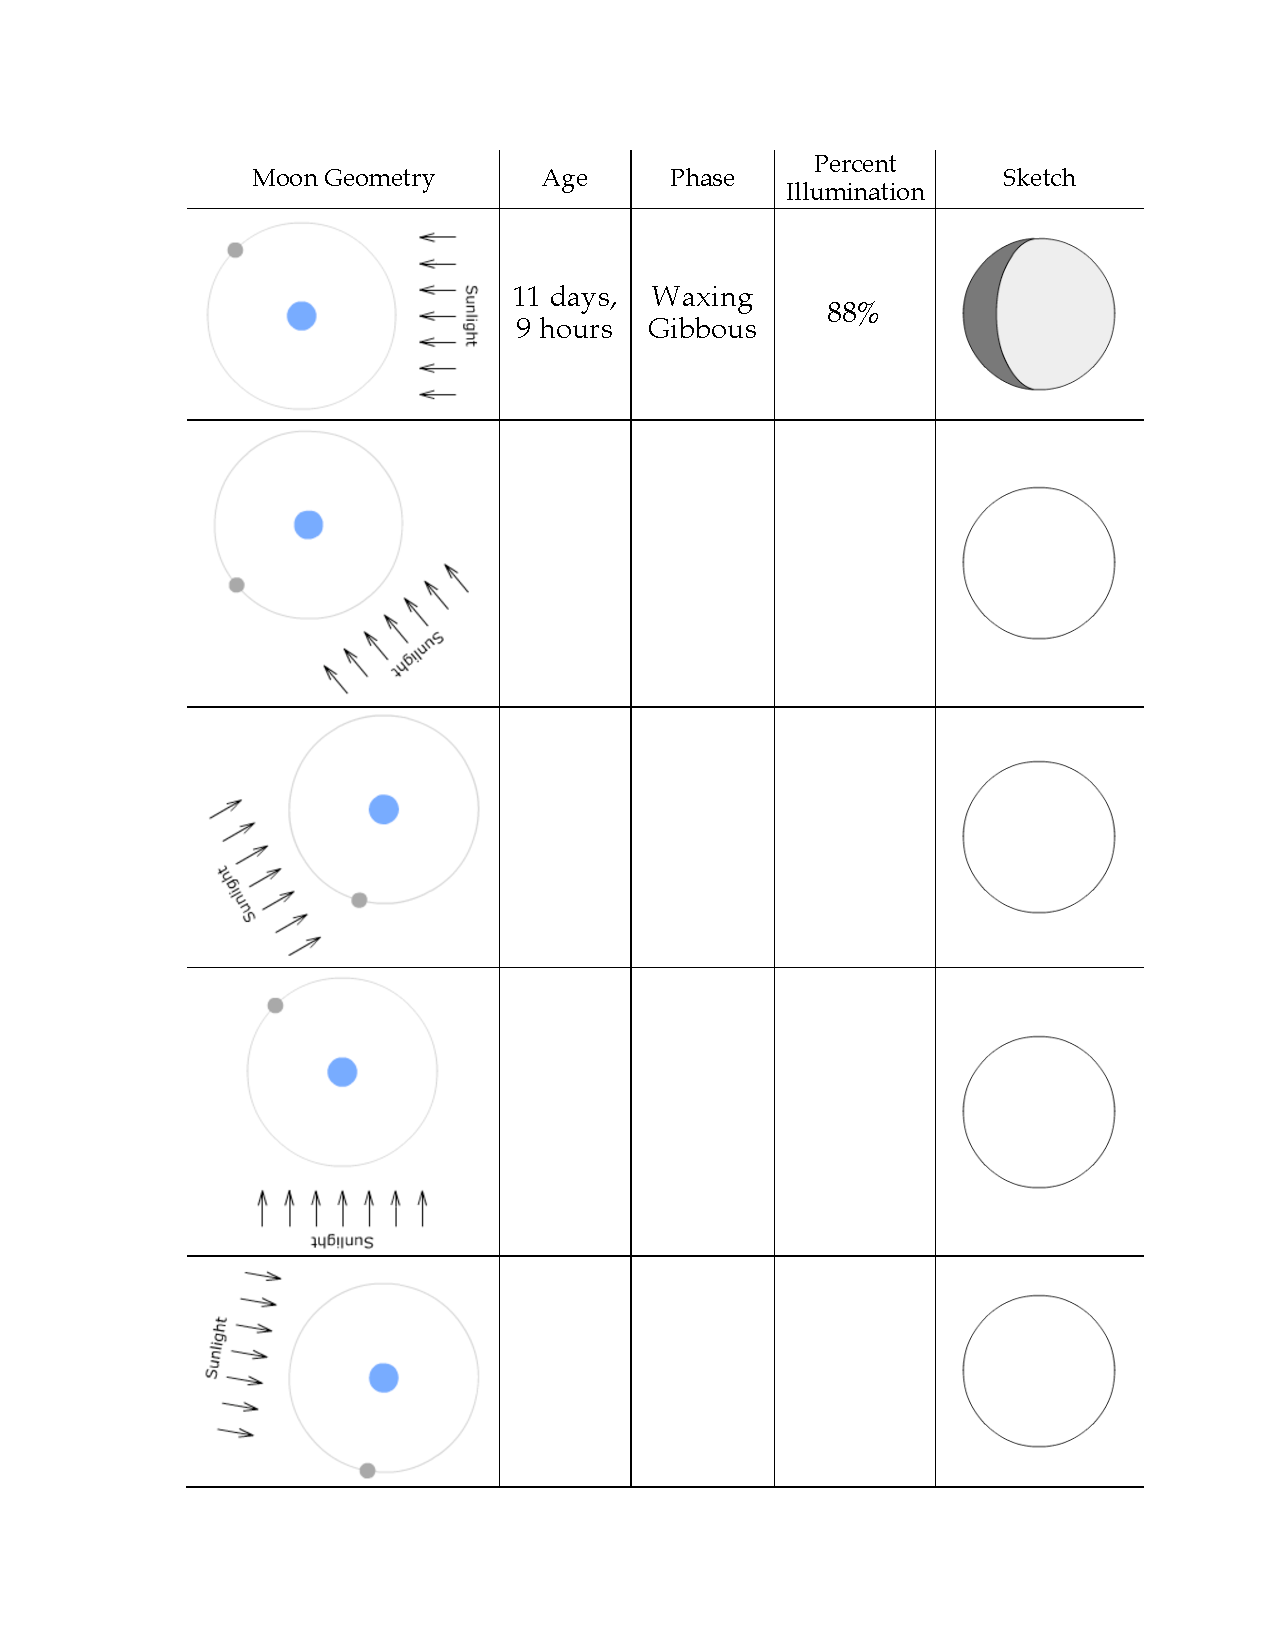
\includepdf{moon_table}


\end{document}



